\documentclass{article}
\usepackage{v-problem}
\vgeometry
\usepackage[shortconst]{physconst}
\begin{document}
\vtitle[ELECTROSTATICS]

\def\pn{02}
\def\book{Irodov}
\def\page{105}
\def\gdrive{
https://drive.google.com/drive/folders/1g0qyA9UnZSR0Ta2VQsGYTPoOP21cLkU5?usp=share_link}

\def\question{
Calculate the ratio of the electrostatic to gravitational interaction forces between two electrons, between two protons. At what value of the specific charge $q/m$ of a particle would these forces become equal (in their absolute values) in the case of interaction of identical particles?
}

\vspace*{\fill}
\begin{tikzpicture}
	\node[qnumber] (n) at (0, 0)[scale=2] {$\pn.$};
	\node[question] (q) [right=2mm of n.east] {\question};
	\tzline[divider]<-0.125, 0> (q.north west)(q.south west);
	\node[format] (f) at  (q.south east){[\book \quad \page]};
\end{tikzpicture}	
\vspace*{\fill}

\begin{center}
\begin{tikzpicture}
\tzcoor*(0,0)(Q1){$e$}[bl](5pt)
\tzcoor*(4,0)(Q2){$e$}[br](5pt)
	\tzline+[->](Q2)(1.5, 0){$F_e$}[r]
	\tzline+[->](Q2)(-1.5, 0){$F_g$}[l]
	
\begin{scope}[yshift=-2cm]
\tzcoor*(0,0)(Q1){$p$}[bl](5pt)
\tzcoor*(4,0)(Q2){$p$}[br](5pt)
	\tzline+[->](Q1)(1.5, 0){$F_g$}[r]
	\tzline+[->](Q1)(-1.5, 0){$F_e$}[l]
\end{scope}
\end{tikzpicture}
\end{center}
\vspace*{\fill}

\pagebreak

\vtitle[\texttt{Solution}]

\addtolength{\jot}{2ex}
\begin{align*}
\intertext{For two electrons}
\dfrac{F_e}{F_g} &= \dfrac{\dfrac{1}{4\pi\varepsilon_0} \cdot \dfrac{q_1q_2}{r^2}}{G \cdot \dfrac{m_1m_2}{r^2}}\\
	&= \dfrac{1}{4\pi\varepsilon_0} \cdot \dfrac{1}{G} \cdot \dfrac{e^2}{m^2}\\
\intertext{Put the numeric values }
\intertext{$k=\kCoulomb, \quad G=\kGravity$}
\intertext{$e=\kChargeFundamental, \quad m_e=\kMassElectron $}	\\
	&\approx 4\times 10^{42} \ans  \\
\end{align*}

\pagebreak
\begin{align*}
\intertext{For two protons}
\dfrac{F_e}{F_g} &= \dfrac{\dfrac{1}{4\pi\varepsilon_0} \cdot \dfrac{q_1q_2}{r^2}}{G \cdot \dfrac{m_1m_2}{r^2}}\\
	&= \dfrac{1}{4\pi\varepsilon_0} \cdot \dfrac{1}{G} \cdot \dfrac{e^2}{m^2}\\
\intertext{Put the numeric values }
\intertext{$k=\kCoulomb, \quad G=\kGravity$}
\intertext{$e=\kChargeFundamental, \quad m_p=\kMassProton $}	\\
	&\approx 1\times 10^{36} \ans  \\
\end{align*}
\pagebreak

\pagebreak
\begin{align*}
\intertext{For $q/m$, if $F_e=F_g$}
F_e &= F_g\\
\dfrac{1}{4\pi\varepsilon_0} \cdot \dfrac{q_1q_2}{r^2} &= G \cdot \dfrac{m_1m_2}{r^2}\\
\dfrac{1}{4\pi\varepsilon_0} \cdot q^2 &= G \cdot m^2\\
\left( \dfrac{q}{m} \right)^2 &= \dfrac{G}{k}\\
\dfrac{q}{m} &= \sqrt{\dfrac{G}{k}}
\intertext{Put the numeric values }
\intertext{$k=\kCoulomb, \quad G=\kGravity$}\\
	&\approx 0.86 \times 10^{-10} C/\kg \ans  \\
\end{align*}
\pagebreak

\vspace*{\fill}
\begin{center}
	\fbox{\qrcode[height=2cm]{\gdrive}}
\end{center}
\vspace*{\fill}

\end{document}
